\section{Requirements}
Zur Spezifikation\todo{Glossar} der Smartwatch wurden - neben den in Abschnitt~\ref{sec:use_cases} beschriebenen UseCases - die wichtigsten Requirements\todo{Glossar} gesammelt und festgehalten. Um die Übersicht und Nachvollziehbarkeit zu verbesseren, werden diese in die folgenden Kategorien eingeteilt:

\begin{itemize}
	\item Ausgabe -- Ausgabe beinhaltet alle Requirements, die sich auf die grafische und auf die akkustische Ausgabe beziehen.
	\item Usability\todo{Glossar} -- Alle Requirements zur Beschreibung der Bedienbarkeit der Smartwatch
	\item Kapazität -- Alle Requirements bezüglich der Energieversorgung
	\item Funktionen -- Funktionen beinhaltet alle Requirements, die konkrete Funktionen der Smartwatch beschreiben
	\item Ergonomie\todo{Glossar} -- Ergonomische Requirements beschreiben das Design und die physische Eigenschaften der Smartwatch.
\end{itemize}

Das Package-Diagram in Abbildung~\ref{fig:package_diagram_requirements} teilt die Requirements-Kategorien in einzelne Packages\todo{Glossar} auf.

\begin{figure}[H]
\centering\
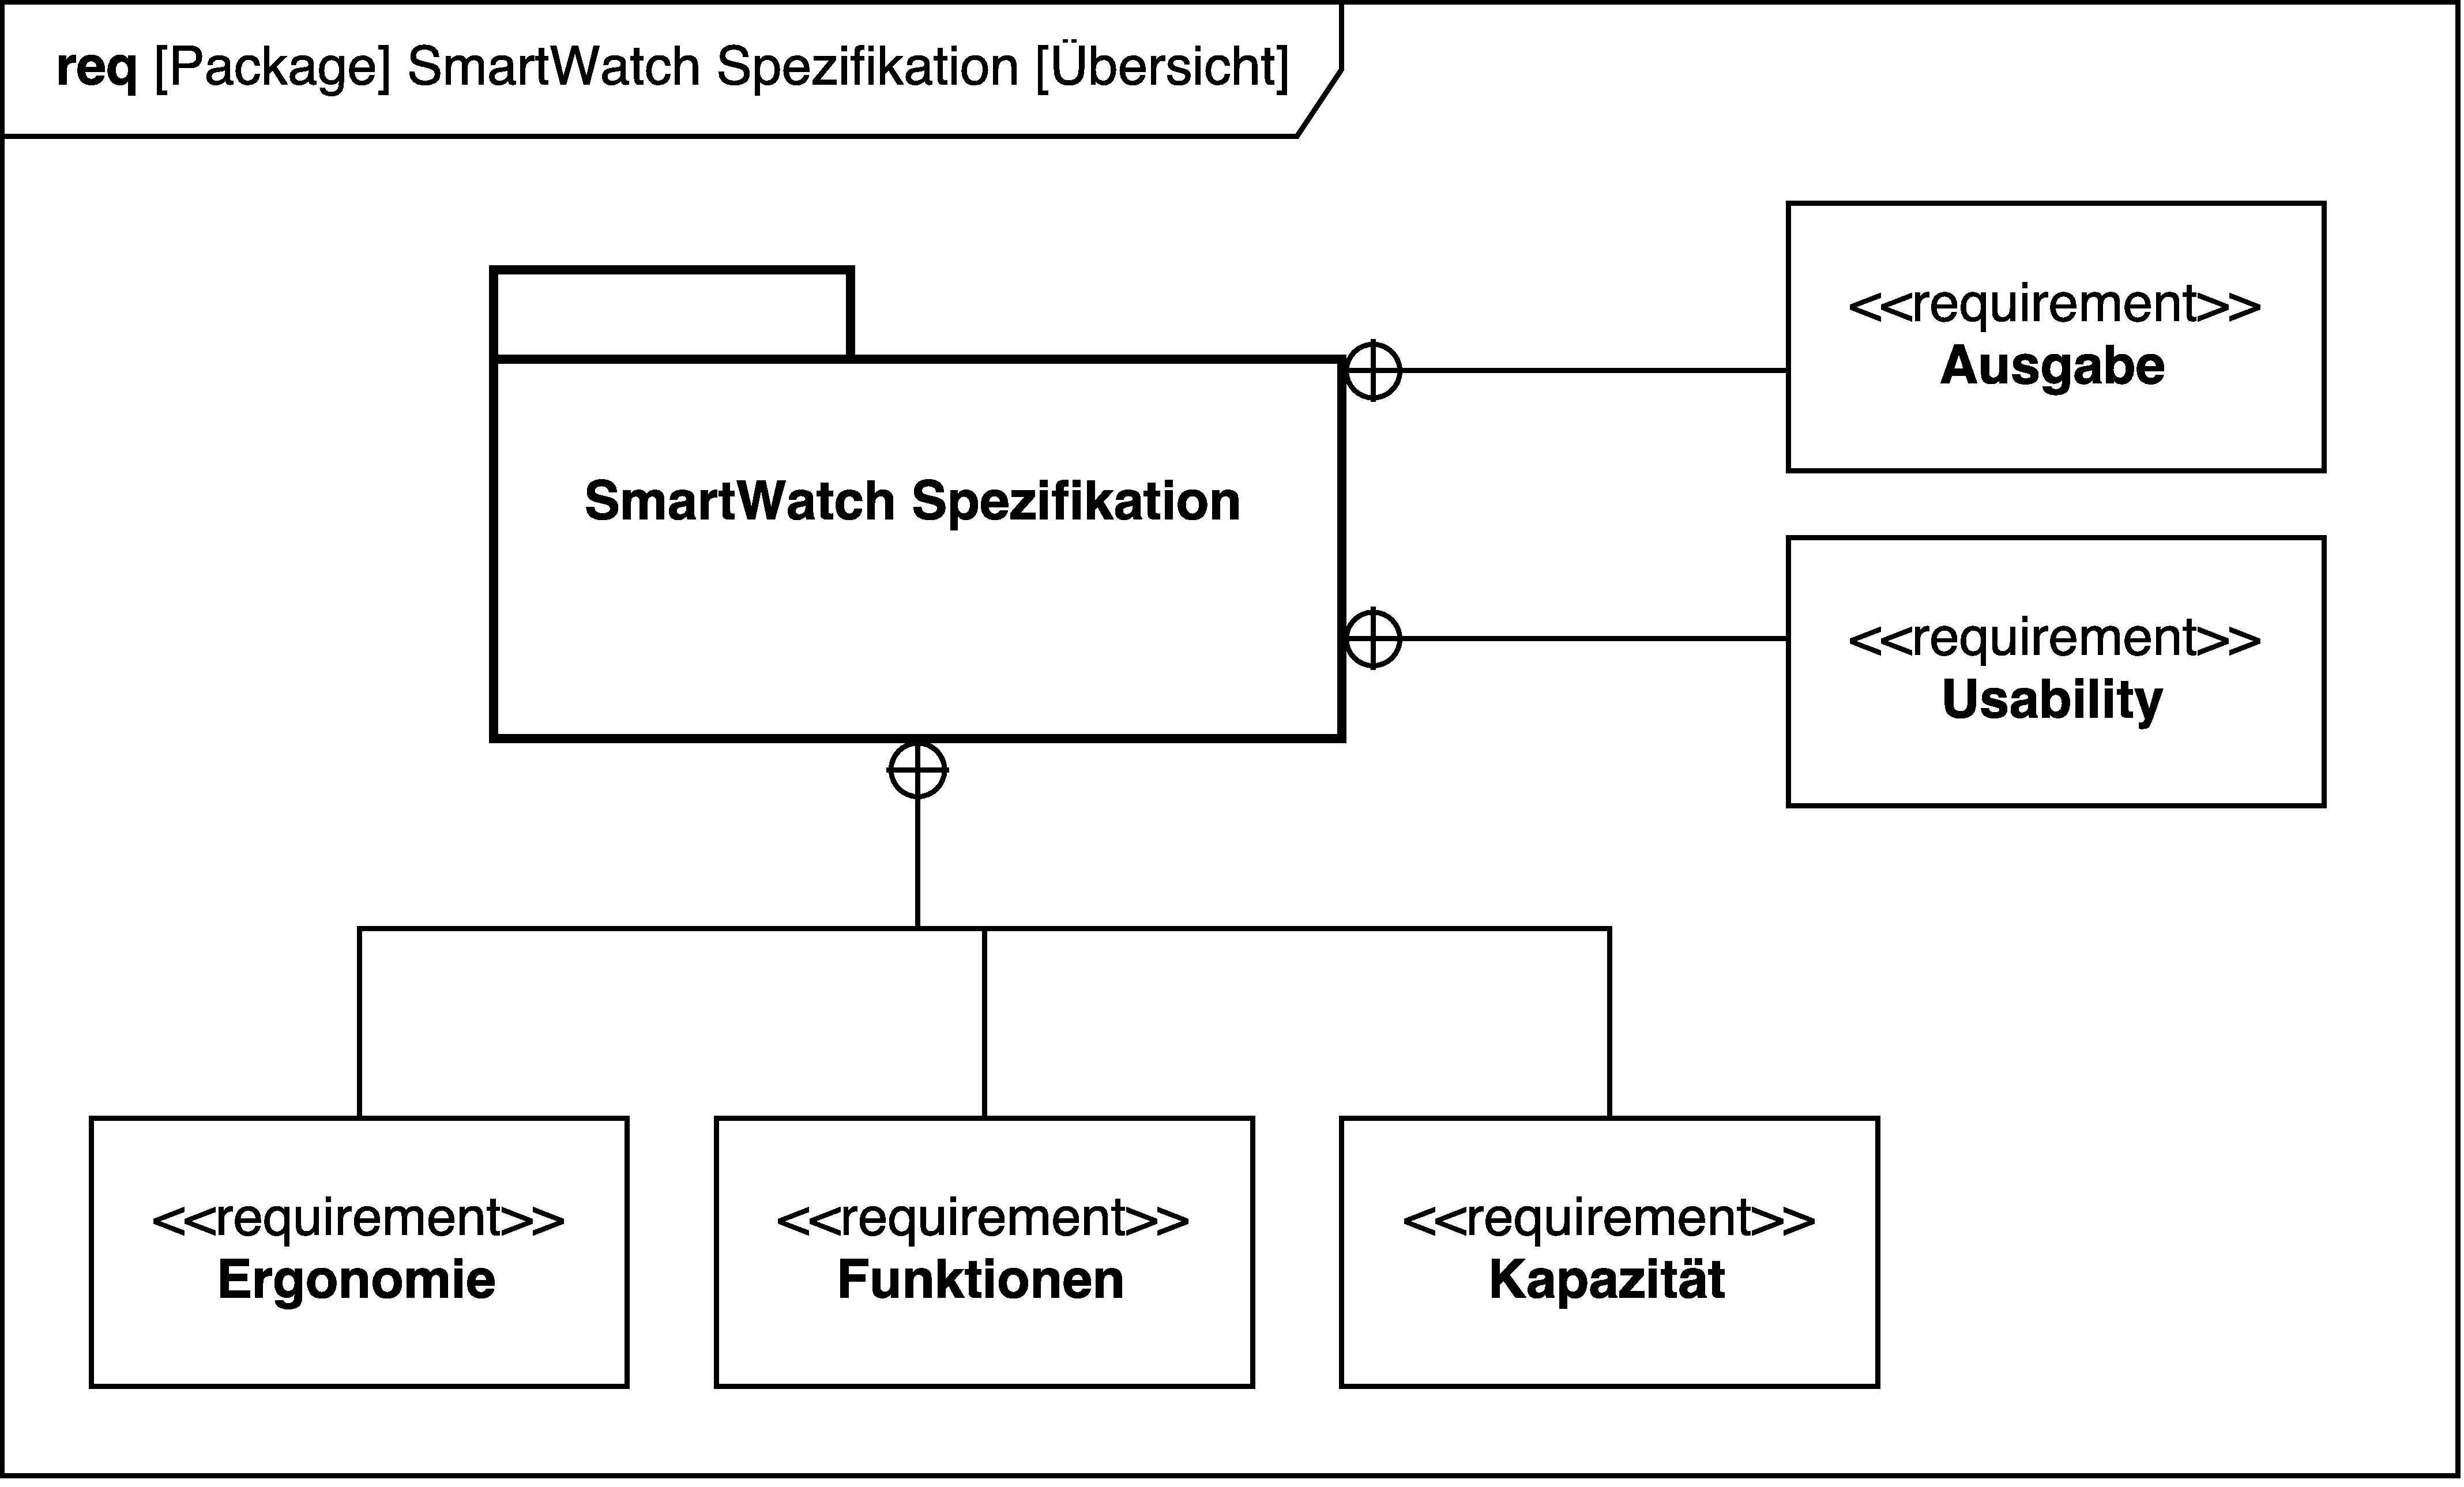
\includegraphics[width=14cm]{img/package_diagram_smartWatch_requirements}
\caption[Requirements: Package Diagram]{Package Diagram der einzelnen Requirement-Kategorien}\label{fig:package_diagram_requirements}
\end{figure}

Tabelle~\ref{tab:table_requirements} enthält die gesammelten Requirements aufgeteilt in die einzelnen Kategorien.

\begin{center}
	\begin{longtable}{|L{2cm}|L{3cm}|L{8.5cm}|}
		\caption[Liste der Requirements]{Auflistung der gesammelten Requirements der Smartwatch} \label{tab:table_requirements} \\
		\hline \multicolumn{1}{|c|}{\textbf{ID}} & \multicolumn{1}{c|}{\textbf{Name}} & \multicolumn{1}{c|}{\textbf{Text}} \\ \hline
		\endfirsthead

		\multicolumn{3}{c}%
		{{\bfseries \tablename\ \thetable{} -- Fortsetzung von vorheriger Seite}} \\
		\hline \multicolumn{1}{|c|}{\textbf{ID}} & \multicolumn{1}{c|}{\textbf{Name}} & \multicolumn{1}{c|}{\textbf{Text}} \\ \hline
		\endhead

		\hline \multicolumn{3}{|r|}{{Fortgesetzt auf der nächsten Seite}} \\ \hline
		\endfoot

		\hline \hline
		\endlastfoot

		%% Ausgabe
		\multicolumn{3}{|l|}{\textbf{Ausgabe}} \\ \hline
		Ausgabe.01 & Displaygröße & Das Display soll eine Auflösung von 500x500 bei einer Bildschirmdiagonale von 4cm besitzen \\ \hline
		Ausgabe.02 & Farbdisplay & Das Display soll Farben darstellen können \\ \hline

		%% Usability
		\multicolumn{3}{|l|}{\textbf{Usability}} \\ \hline
		Usability.01 & Sichtbare Symbole &	Symbole sollten auf dem Display gut erkennbar sein \\ \hline
		Usability.02 & Touch-Symbolgröße &	Symbole, die eine Touch-Funktionalität besitzen, müssen mindestens 75\% des Bildschirms einnehmen \\ \hline

		%% Kapazität
		\multicolumn{3}{|l|}{\textbf{Kapazität}} \\ \hline
		Akku.01 & Akkulaufzeit & Eine Akkuladung soll bei normaler Benutzung mindestens 24 Stunden halten \\ \hline
		Akku.02 & Akkuladezeit & Der Akku soll innerhalb von 2 Stunden vollständig geladen werden \\ \hline
		Akku.03 & Induktionsladen & Der Akku soll über Induktion (z.B. Qi-Standard) geladen werden können \\ \hline

		%% Funktionen
		\multicolumn{3}{|l|}{\textbf{Funktionen}} \\ \hline
		Boot.01 & Bootvorgang maximal 10 Sekunden & Der Bootvorgang der Smartwatch soll maximal 10 Sekunden dauern \\ \hline
		Connection.01 &	Verbindung mit Smartphone & Das System soll sich mit einem Smartphone verbinden können \\ \hline
		Wasserdicht.01 & Wasserdicht bis 30 Meter & Das System soll Wasserdicht bis 30 Meter sein \\ \hline
		Notification.01 & Anzeigen der Notifications & Notifications sollen auf der Uhr angezeigt werden \\ \hline
		Notification.02 & Notifications innerhalb einer Sekunde anzeigen & Notifications sollen maximal nach einer Sekunde auf der Uhr angezeigt werden \\ \hline
		Connection.02 &	Verbindung mit Smartphone in 4 Sekunden & Die Verbindung mit dem Smartphone  muss in maximal 4 Sekunden hergestellt werden \\ \hline

		%% Ergonomie
		\multicolumn{3}{|l|}{\textbf{Ergonomie}} \\ \hline
		Ergonomie.01 & Auswechselbares Armband & Das Armband der Uhr soll ausgewechselt werden können \\ \hline
		Ergonomie.Gewicht.01 & Gesamtgewicht & Das Gesamtgewicht der Uhr soll maximal 50 Gramm wiegen \\ \hline

	\end{longtable}
\end{center}
